\chapter{Atmel AVR}\label{atmel-avr}

\section{Introduction}\label{avr-introduction}

The Atmel AVR is the micro controller at the heart of your \indexasis{Arduino} and comes in many different varieties. We are concentrating, in the main, on the Atmel ATmega328P which is the micro controller on the Duemilanove, the UNO and the Nano - although the Nano uses a surface mount version of the 328.

Some clones may also use the surface mounted version of the 328 - it depends. The \indexasis{Arduino} hardware is open source, so anyone is able to build their own clones, using whatever equivalent micro controllers they can source.

\section{Data Sheets}\label{data-sheets}\index{Data Sheets}

You should, if you have not already done so, download the full data sheet for the ATmega320P from \href{http://www.atmel.com/Images/Atmel-42735-8-bit-AVR-Microcontroller-ATmega328-328P_Datasheet.pdf}{Atmel's web site} - don't worry about the fact that the document is over 440 pages long, we \emph{won't} be reading it from start to finish!

Normally, it's good to get an overview of the micro controller, especially when it's new to us, by reading  through the first few chapters which describe the micro controller and it's registers and features etc.

We will not labour the point here. The data sheet contains all you need to know, and much, much more. 

\section{ATmega328P Pinout}\label{atmega328p-pinout}
Figure~\ref{fig-atmega328p-pinout}, taken from the current data sheet,  shows details of the ATmega328P's various pins. You will notice that there is no mention of the \indexasis{Arduino}'s pins D0 through D13, nor of pins A0 through A5, so perhaps Figure~\ref{fig-arduino-uno-pinout} will help, as the \indexasis{Arduino} pin usage is shown in red text down each side of the diagram. (Image courtesy of \href{https://www.arduino.cc/en/Hacking/PinMapping168}{www.arduino.cc})

\begin{note}
	You will note that Figure~\ref{fig-arduino-uno-pinout} mentions the \indexasis{ATmega168} rather than the \indexasis{ATmega328P} - don't worry, they are pin compatible. The pins on one micro controller are the same, and have the same functions, as those on the other. They just have different amounts of memory - flash, EEPROM and SRAM.
\end{note}	

\begin{figure}[p]
	\centering
	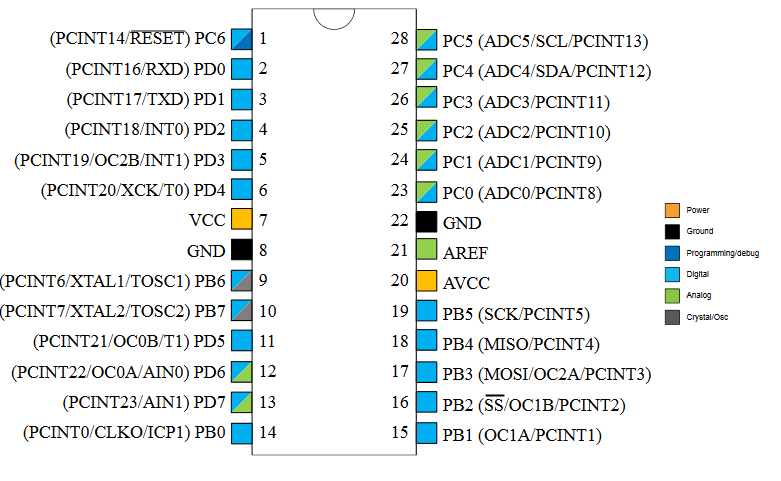
\includegraphics[width=0.9\textwidth]{Content/images/ATmega328P-pins}
	\caption{Pinout Diagram of the ATmega328P Micro Controller}
	\label{fig-atmega328p-pinout}
\end{figure}

\begin{figure}[p]
	\centering
	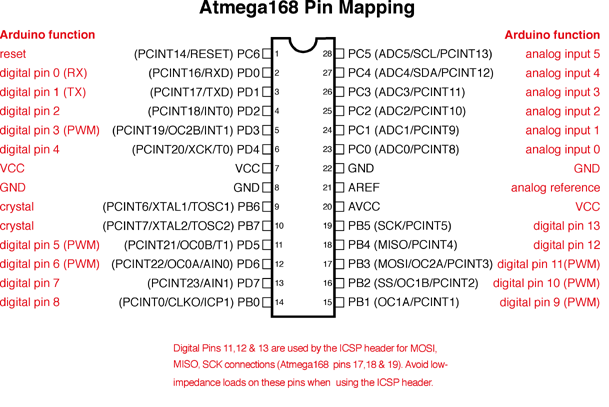
\includegraphics[width=0.9\textwidth]{Content/images/ArduinoUno-pins}
	\caption{Pinout Diagram of the ATmega328P showing Arduino Pin Use}
	\label{fig-arduino-uno-pinout}
\end{figure}

You may be wondering how, if the AVR pinout diagram shown in Figure~\ref{fig-atmega328p-pinout} doesn't have the Arduino's pin definitions, how the Arduino software is able to use the correct pins? This will be explained in section~\refname{avr-pinmodes} on page~\pageref{avr-pinmodes}.

\section{AVR Pinmodes}\label{avr-pinmodes}

You are most probably familiar with the \indexasis{Arduino}'s \inline{pinMode()} function, which allows you to define whether a pin is to be configured as input, output or input with pullup. You will not be surprised to find out that the AVR has a similar feature, but this one can do many pins at once.

However, as mentioned above, you may be wondering how the  \indexasis{Arduino} software gets from the \indexasis{Arduino} pin numbering format to those used on the actual AVR hardware? The process  as followed by \inline{pinMode()}, is as follows:

\begin{itemize}
	\item Convert the pin number to a \emph{bit mask} by calling \inline{digitalPinToBitMask()}.
	\item Convert the pin number to a port as well, by calling \inline{digitalPinToPort()}. If the port is invalid, do nothing and exit.
	\item Convert the (valid) port to a mode register by calling \inline{portModeRegister()}.
	\item Convert the (valid) port to a port output register by calling \inline{portOutputRegister()}.
	\item Preserve the current status register for the micro controller. Amongst other details, this will record the current state of the interrupts - whether or not they are currently enabled\footnote{See the data sheet for details of what the Status Register contains.}.
	\item Turn off any interrupts, even if already off. See \href{http://code.google.com/p/arduino/issues/detail?id=146}{This issue} for details of why this has to be done.
	\item Set the pin according to the desired mode - INPUT, INPUT\_PULLUP or OUTPUT.
	\item Restore the status register. This will also re-enable the interrupts, if they were enabled earlier.
\end{itemize}

That's an awful lot of work just to set a pin as OUTPUT, for example.

The functions \inline{digitalPinToBitMask()}, \inline{digitalPinToPort()}, \inline{portModeRegister()} and \inline{portOutputRegister()} are defined in the file:

\fbox{\inline{hardware/avr/cores/arduino/Arduino.h}}

which is located underneath wherever your \indexasis{Arduino} software is installed. If you ()only) have \indexasis{PlatformIO} installed, then the definitions are in:

\fbox{\inline{/home/norman/.platformio/packages/framework-arduinoavr/cores/arduino/Arduino.h}}

So, how does all of the above get us from the pin number 13, for pin D13, for example, to PB5? Well, the next section explains Ports and Pins, but briefly, calling \inline{pinMode(13, OUTPUT)} does all of the following:

\begin{itemize}
	\item \inline{digitalPinToBitMask(13)} returns a binary value of 0010 000, which is an 8 bit value, with bit 5 set to 1 and all other bits set to 0.
	\item \inline{digitalPinToPort(13)} returns the value 2, which is defined as a constant named ``PB''.
	\item \inline{portModeRegister(PB)} returns a pointer, this is C code remember, to the ``DDRB'' register. More on this in the following section.
	\item \inline{portOutputRegister(PB)} returns a pointer to ``PORTB''. More below on this too.
	\item Saves the status register.
	\item Turns off interrupts.
	\item Binary ORs the required bit of the ``DDRB'' register, bit 5 as above, with a 1, to set the pin to an output.
	\item Restores the status register (and interrupt state).
\end{itemize}

As I said, that's a lot of work, and a lot of code. In addition, there are a number of data tables written to the flash memory, where your program lives, to enable the above function calls to be facilitated. These tables take up $(3 * 10) + (3 * 20)$ or 90 bytes of potentially valuable program space.

That's for the \indexasis{Arduino}. For plain AVR C code, we set D13 (aka PortB, Pin 5) as follows:

\begin{lstlisting}[numbers={none}]
	DDRB |= (1 << 5);
\end{lstlisting}

Which is a lot less work, a lot fewer bytes overall and no tables are required. However, \emph{we}, the programmer, do have to remember the pin numbers etc.

The following section goes into greater detail about Pins and Ports.

\section{AVR Ports and Pins}\label{avr-ports-and-pins}

\subsection{Ports}\label{avr-ports}

The \indexasis{ATmega328P} has three separate ports named B, C and D. Other devices in the AVR family have additional ports, but we are restricted to the three already mentions.

The ports are named, simply enough, ``PORTB'', ``PORTC'' and ``PORTD''. Normally, each port will control up to 8 individual GPIO  pins, but on an Arduino, not all ports have the full set on pins.

A port, internally to the AVR, is simply an 8 bit register/memory address, connected via some complicated electronics, to the physical pins on the outside of the chip.

As far as we AVR and Arduino programmers, are concerned, we have the following ports (and therefore pins) available:

\begin{itemize}
	\item PORTB bits 0 to 5 = PB0 to PB5 = Arduino pins D8 to D13.
	\item PORTB bits 6 and 7 = PB6 and PB7. On the Arduino, these are used for the 16Mhz crystal and are not available as GPIO pins. Home brew setups can, if required, run off the micro controller's internal clock, and will be able to use these two pins.
	\item PORTC bits 0 to 5 = PC0 to PC5 = Arduino analogue pins A0 to A5.
	\item PORTC bit 6 = PC6 = the reset pin and, while it \emph{can} be fused as a GPIO pin, it is not usually configured in this manner. Doing so also disables the ability to reprogram the chip - unless you have a high voltage programmer. Best avoided!
	\item PORTD bits 0 to 7 = PD0 to PD7 = Arduino pins D0 to D7.
\end{itemize}

\subsubsection{Writing to an Output Port}\label{avr-ports-output-writing}
Writing a binary 1, to a bit in PORTx\footnote{The `x' refers to `B', `C' or `D'.} will set the connected GPIO pin high, if the pin is configured as an output of course. If it is configured as in input, writing a 1 will actually enable the input pullup resistor for  that pin.

\begin{lstlisting}[language=C,numbers={none}]
	// I want the  LEDs on PB5 to switch on, everything else off.
	PORTB = (1 << PB5);
}
\end{lstlisting}


\subsection{Pins}\label{avr-pins}

As mentioned above, each port in an AVR micro controller controls up to 8 GPIO pins. 

These GPIO pins can be configured as ``INPUT'', ``INPUT with PULLUP'' or ``OUTPUT''. 

In order to do this, there's a special register named the Data Direction Register, or ``DDR'' for each port. PORTA has DDRA, PORTB has DDRB and so on.

\subsubsection{Output Pins}\label{avr-pins-output}
In order to configure the pin PB5 (aka \indexasis{Arduino} D13) as an output, we set bit 5 to a 1. To configure as an input, we reset bit 5 of DDRB to a zero. You have seen the use of DDRB previously, in listing~\ref{lst-avrblink.c} where we did the following:

\begin{lstlisting}[language=C,numbers={none}]
	DDRB = (1 << PB5);
\end{lstlisting}

We could have also done the same thing as follows:

\begin{lstlisting}[language=C,numbers={none}]
	DDRB = (1 << DDB5);
\end{lstlisting}

or even:

\begin{lstlisting}[language=C,numbers={none}]
	DDRB = (1 << PORTB5);
\end{lstlisting}

This is because when we compile code for an \indexasis{ATmega328P}, there are certain values defined for us, and all of the above are defined as 5. They have different uses, but most AVR code that I've seen, uses the first version above. So I'll (probably) stick with that too. Feel free to use whatever version you are most comfortable with.

\begin{note}
	In general, if you want to set a bit in a register, or whatever, you can also use the \inline{\_BV} macro. This causes the \emph{compiler} to convert something like \inline{\_BV(5)} into \inline{(1 << 5)} but it is done at compile time so has no overhead at runtime.
	
	This means that there's another version of the code above to set bit 5 in DDRB, and that is:
	
	\begin{lstlisting}[language=C,numbers={none}]
		DDRB = _BV{5};	\end{lstlisting}	
\end{note}	

Of course, every version of the above is slightly incorrect. We do set bit 5 as desired, but we also reset all the other bits. This might affect your device especially as it may have already set some other bits to indicate output pins.

What we should have done is to binary ``OR'' the required pin values into the existing value in the DDR register, as follows:

\begin{lstlisting}[language=C,numbers={none}]
	DDRB |= (1 << PB5);
\end{lstlisting}

This will now \emph{only} affect bit 5, all the other bits remain unchanged.

We can set multiple pins as output, in the same command, as follows:

\begin{lstlisting}[language=C,numbers={none}]
	DDRB |= (1 << PB5)  | (1 << PB3);
\end{lstlisting}

Which will set pins PB3 and PB5 as outputs without affecting  the other pins.

\subsubsection{Input Pins}\label{avr-pins-input}

So far, we have seen how to set pins as output, equivalent to the \indexasis{Arduino}'s \inline{pinMode(pin, OUTPUT)} command. How then do we set a pin as input?

When the AVR is powered on, or reset, then the default setting for all pins is as input. However, it's best to be explicit. You could do this to set all the pins on PORTB to input mode:

\begin{lstlisting}[language=C,numbers={none}]
	DDRB = 0;
\end{lstlisting}

You could, but again, you are possibly reconverting some pins that have been set as outputs, elsewhere in your code. (Ask me how I know!) The best way is simply to binary ``AND'' a zero into the desired pin position, as follows:

\begin{lstlisting}[language=C,numbers={none}]
	DDRB &= ~(1 << PB5);
\end{lstlisting}

This creates a value with bit 5 set to a 1, and all other bits reset to zero, then flips it around so that all bits are set to 1 except bit 5. This is then ANDed with the current value in DDRB which has the effect of resetting bit 5 of DDRB to a zero, without affected any other bit.

As above, we can set multiple pins to be inputs quite simply:

\begin{lstlisting}[language=C,numbers={none}]
	DDRB &= ~((1 << PB5) | (1 << PB3));
\end{lstlisting}

This will set pins PB3 and PB5 as inputs without affecting other pins.

Ok, I hear you ask, we have output and input using a single bit per pin, so how do we get INPUT\_PULLUP like the \indexasis{Arduino}?

It was mentioned in passing above, but this is all you have to do:

\begin{itemize}
	\item Set the pin as an input in the normal manner.
	\item Write a 1 to the corresponding bit of the pin's PORTx register.
\end{itemize}

So, to set PB3 to an input, with pullup enabled, all we have to do is this:

\begin{lstlisting}[language=C,numbers={none}]
	// Configure PB3 as an input pin first.
	DDRB &= ~(1 << PB3);
	
	// Enable the pullup resistor on PB3.
	PORTB |= (1 << PB3);
\end{lstlisting}


\subsubsection{Reading From an Input Port}\label{avr-ports-input-reading}

To read the value of the pins configured as input, you simply read the value from the PINx\footnote{The `x' refers to `B', `C' or `D'.} register, for example:

\begin{lstlisting}[language=C,numbers={none}]
	uint8_t inputPins = PINB;
	if (inputPins & (1 << PB5)) {
		// Do something if pin PB5 is high.
	}
\end{lstlisting}


If a particular input pin is connected to ground (0 Volts) then the corresponding bit in the PINx register will be a zero. If a pin is connected to a \emph{high} voltage, then it will show a 1 in the corresponding bit of the appropriate PINx register.

Input pins with pullup\footnote{% complicated footnote ahead!
	I don't know about you, but I find it strange that a switch, for example, that is closed, returns a logical zero to the micro controller, rather than a 1 - which to me makes a lot more logical sense. Still, pullups! I would rather configure the pin as an input, with no pullup, and use an external \emph{pulldown} resistor to ground myself. That way, an open switch gives a zero bit in the appropriate PINx register, while a closed switch gives a 1. Or is that just me? 
	
	Yes, I \emph{know} that would be an additional cost when lots of pulldown resistors were required, in a commercial product, but I'm not making commercial products, and I have a bucket of resistors to use up!%
} will, of course, show a 1 unless pulled to ground by some external circuitry.




